\documentclass[11pt,a4paper]{article}
\usepackage[spanish]{babel}
\usepackage[utf8]{inputenc}
\usepackage[top=2cm, bottom=2cm, left=2cm, right=2cm]{geometry}
\usepackage{commath,amsmath,lastpage,float,sectsty,hyperref,graphicx,pdfpages,fancyhdr,listings,siunitx}

\sectionfont{\fontsize{12}{15}\selectfont}
\linespread{1.25} % Interlineado 1.5
\renewcommand{\rmdefault}{phv} % Arial
\renewcommand{\sfdefault}{phv} % Arial

\hypersetup{
    pdftitle={Trabajo Práctico 1},
	pdfsubject={Análisis Numérico I},
	pdfauthor={del Mazo Federico, Kristal Juan Ignacio},
}

\lstset{
  basicstyle=\ttfamily,
  columns=fullflexible,
  frame=single,
  breaklines=true,
  postbreak=\mbox{\textcolor{red}{$\hookrightarrow$}\space},
}

\fancypagestyle{enunciado}{
    \fancyhf{}
    \fancyhead[C]{Enunciado provisto por la catedra}
}

\pagestyle{fancy}
\fancyhf{}
\fancyhead[R]{Trabajo Práctico 1 - 2018c2}
\fancyhead[L]{75.12 Análisis Numérico I}
\renewcommand{\headrulewidth}{0.4pt}
\fancyfoot[L]{100029 - 99779}
\fancyfoot[R]{\thepage de \pageref*{LastPage}}
\renewcommand{\footrulewidth}{0.4pt}
\setlength{\footskip}{17pt}

\fancypagestyle{onlyheader}{
\fancyfoot{}
}

\begin{document}

\begin{titlepage}
	\hfill
\includegraphics[width=6cm]{figuras/fiuba.jpg}
    \begin{center}
    \vfill
    \Huge \textbf{Trabajo Práctico 1}
    \vskip2cm
    \Large [75.12] Análisis Numérico I\\
    Segundo cuatrimestre de 2018
    \vfill
    \begin{tabular}{|l|c|r|}
	\hline
	Alumno & Padrón & Mail\\
	\hline
	\hline
	del Mazo, Federico & 100029 & delmazofederico@gmail.com\\
	\hline
	Kristal, Juan Ignacio & 99779 & kristaljuanignacio@gmail.com\\
	\hline
	\end{tabular}
    \vskip2cm
    \end{center}

    Curso 07:

    \begin{itemize}
    \item Dr Daniel Fabian Rodriguez
    \item Valeria Machiunas
    \item Federico Balzarotti
    \item Michael Portocarrero
    \end{itemize}

\end{titlepage}

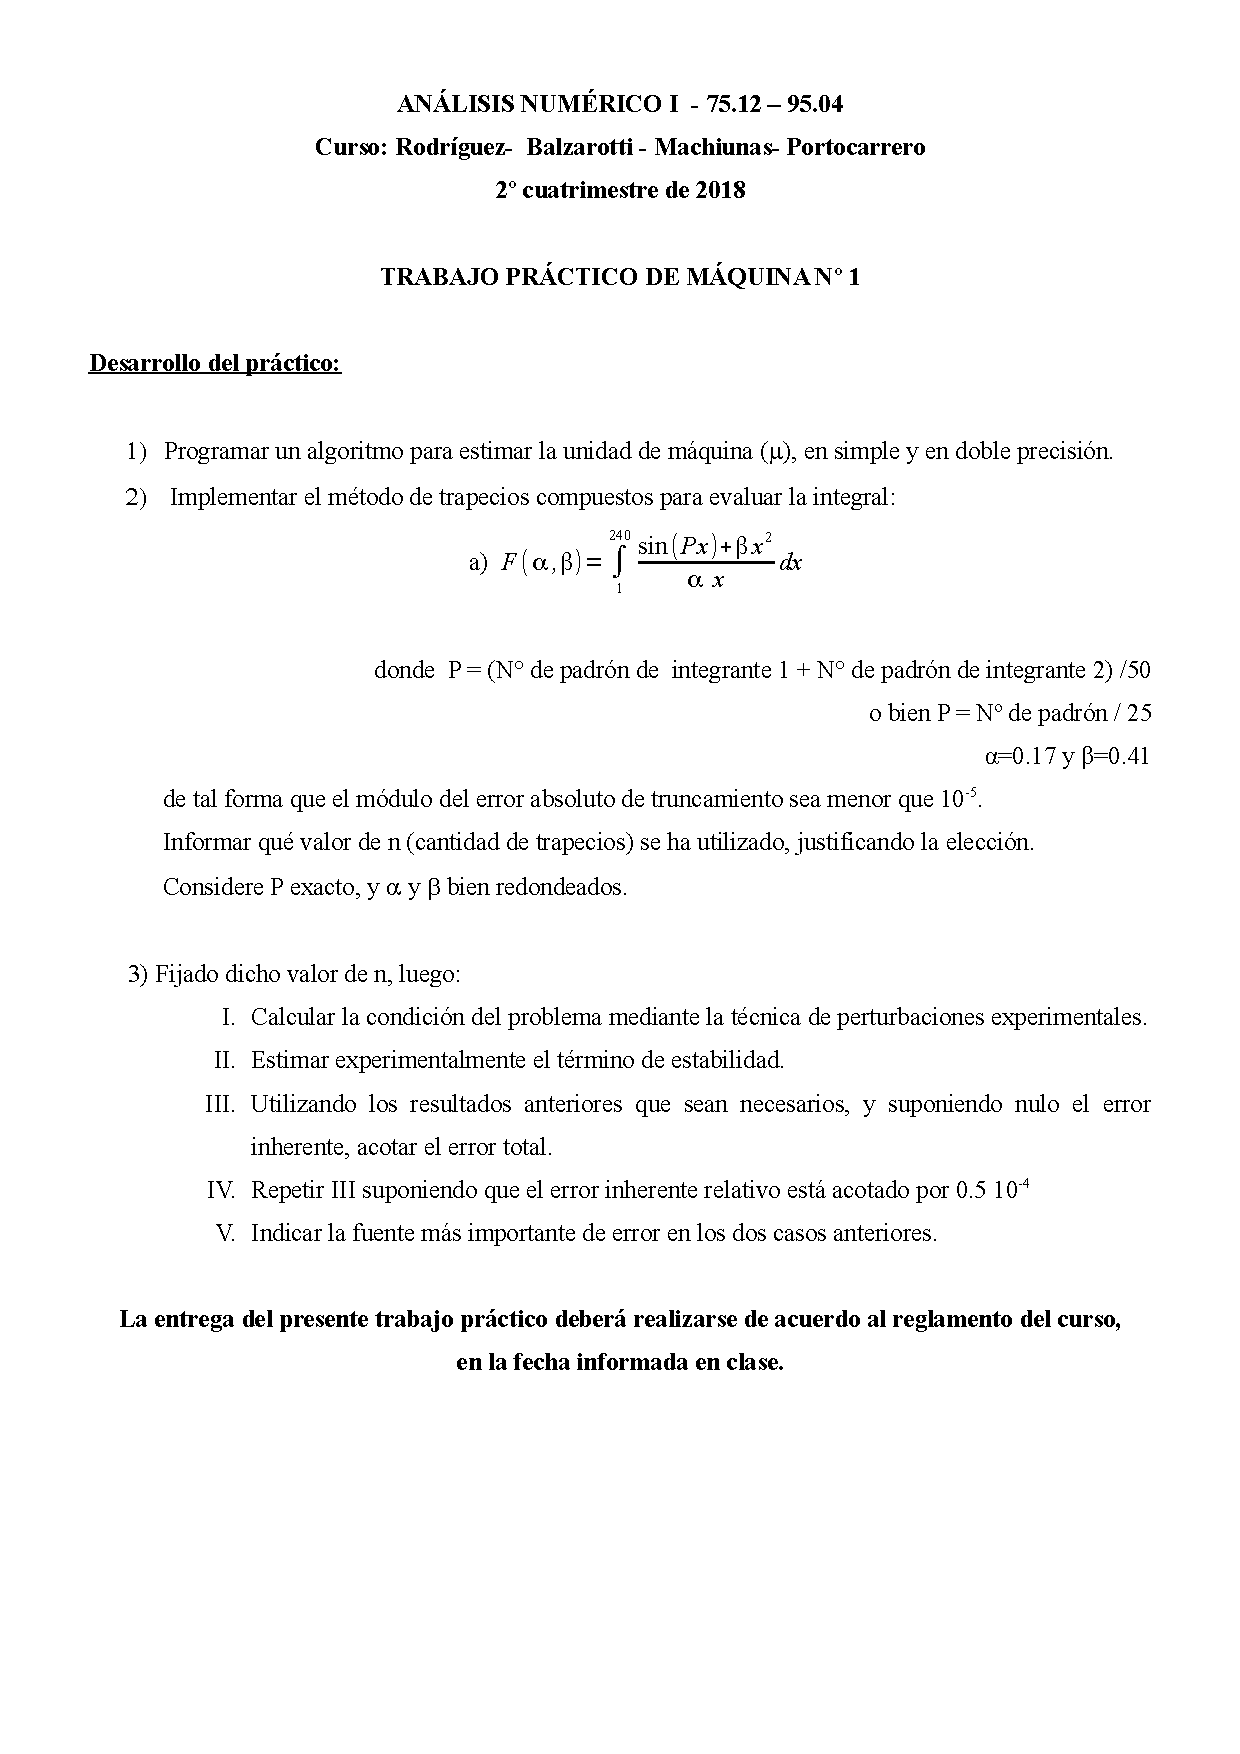
\includepdf[pages=-,pagecommand={\thispagestyle{enunciado}}]{TP1-Enunciado.pdf}

\pagenumbering{gobble}
\tableofcontents
\thispagestyle{onlyheader}
\newpage

\pagenumbering{arabic}
\setcounter{page}{1}

\section{Introducción}
El trabajo práctico tiene como objetivo el cálculo y acotamiento de errores de la siguiente integral:

\[ F(\alpha,\beta) = \int_{1}^{240}  \frac{\sin{(P x)}  + \beta x^2}{\alpha x} dx \]

Siendo:
\begin{itemize}
\item \( P = \frac{\sum\limits_{padrones}^{}}{50} = \frac{99779 + 100029}{50} = 3996.16 \) exacto 
\item \( \alpha = 0.17 \) bien redondeando
\item \( \beta = 0.41 \) bien redondeando
\end{itemize}

Específicamente:

\begin{itemize}
\item Se estimará el valor de la unidad de maquina \( \mu \).
\item Se evaluará la integral con el método de trapecios compuestos teniendo con objetivo en mente que el error absoluto de truncamiento sea menor a \num{1e-5}.
\item Se calculará computacionalmente la cantidad de trapecios utilizada en el método descrito anteriormente.
\item Se calculará la condición del problema mediante perturbaciones experimentales.
\item Se estimará experimentalmente el término de estabilidad.
\item Se acotará el error total.
\end{itemize}

\section{Desarrollo}

\subsection{Estimación de \( \mu \) }

Para los cálculos del \( \mu \) se utilizó el algoritmo del ejemplo 6.4 del libro de Hernan Gonzales \cite{Gonzales}.

\subsection{Función y sus derivadas}

Siempre teniendo en cuenta los valores de \(P, \alpha, \beta \) previamente utilizados, definimos la funcion \( f(x) \) como:

\[ f(x) = \frac{\sin{(P x)}  + \beta x^2}{\alpha x} \]

Graficamos la función para saber un poco más de ella en la figura \ref{fig:funcion}



De esta función calculamos sus derivadas y las graficamos en las figuras \ref{fig:funcionderivada} y \ref{fig:funcionderivada2}, para utilizar en cálculos posteriores.

\[ f'(x) = \frac{P \cos{(P x)}}{\alpha x} - \frac{ \sin{(P x)}}{\alpha x^2} + \frac{\beta}{\alpha} \]

\[ f''(x) = - \frac{2 P \cos{(P x)}}{\alpha x^2} + \frac{2 \sin{(P x)}}{\alpha x^3} - \frac{P^2 \sin{(P x)}}{\alpha x}\]

\subsection{Método de trapecios compuestos}

Sabemos que el error de truncamiento producido por el método de trapecios compuestos es:

\[ \epsilon_t = - \frac{{(b - a)}^3}{12 n^2} * f''(\xi) \]

Donde \(b, a\) son los limites de integración y \(n\) es la cantidad de trapecios. Como lo que queremos es acotar el error de truncamiento, debemos evaluar a la segunda derivada en su imagen máxima, es decir \(\xi = 1 \).

Por lo tanto, y ahora con el error de truncamiento al que queremos llegar, despejamos la cantidad de trapecios:

\[ n = \sqrt{ \abs{ - \frac{(b - a)^3 * f''(1)}{12 \epsilon_t}}} \]

Es con este n que se puede finalmente implementar la función de el método de los trapecios compuestos.

\subsubsection{Truncamiento de n}

Al despejar por el método de los trapecios compuestos el n necesario para tener el error deseado se notó que este valor era de tal magnitud y orden que computacionalmente carecería de sentido usarlo para cada cálculo. Es por esto que se decidió hacer un truncamiento de este valor, para poder tratarlo como es debido y en un lógico margen de tiempo. De todas formas, solo anecdóticamente, se incluye una corrida del programa con el n original.

El criterio para truncar n es el de ver como escala el cálculo de la integral respecto del valor, y luego decidir un punto de corte tratable arbitrariamente (en nuestro caso, 5 minutos). Se puede ver en el gráfico \ref{fig:calcularn} que esta es una función lineal, lo cual tiene sentido ya que lo único que adiciona computacionalmente es el ciclo definido \texttt{for} de la función, haciendolo \(\mathcal{O}(n)\), siendo n el mismo n con el que venimos tratando, redundantemente.

\subsection{Condición del problema y término de estabilidad}

Para realizar las perturbaciones lo haremos sobre alpha y beta respectivamente, introduciendo un error en un ciclo de 16 iteraciones. Una vez obtenidos distintos resultados y teniendo en cuenta el primer valor obtenido, calculamos la nueva condición del problema, una por iteración. Finalmente, de todos los CP obtenidos, tomamos el mayor, tanto para alpha como para beta y es ese nuestro resultado final.

Es ahora que, teniendo en cuenta los valores de la integral con precisión simple y precisión doble (utilizando el valor de n no truncado, para poder apreciar de manera mas exagerada la inestabilidad del algoritmo) podemos calcular el valor del término de estabilidad. Esto lo hacemos con la siguiente ecuación:

\[ Te = \frac{integral_doble - integral_simple}{integral_doble*\mu_s} \]

Finalmente, se grafica en la figura \ref{fig:cpsa} y la figura \ref{fig:cpsb} el cálculo del Cp respecto de alpha y beta en cada iteración.


\subsection{Error total}

Sabiendo que el error total es la sumatoria de los errores inherentes, de redondeo y de truncamiento querémos ahora acotar el error total.

\[ Et = Ei + Er + Etr \]

\[ Et = Cp * r + Te * \mu_s + Etr \]

Este cálculo lo haremos con dos casos en particular:

\begin{itemize}
\item Error inherente nulo
\item Error inherente acotado
\end{itemize}

\subsection{Fuentes de error}

Se puede observar en ambos casos que la mayor fuente de error es el error de redondeo, y esto tiene sentido de acuerdo al método empleado. Al efectuar el metodo de trapecios compuestos se requieren computar muchisimas sumas y multiplicaciones, cada una con sus respectivos errores de redondeo los cuales son variantes en base al error de maquina particular utilizado. Considerando el alto valor de n calculado, la cantidad de sumas es extremadamente grande y por lo tanto el error toma un valor incluso mayor al de truncamiento para dicho n. Todo esto considerando al n original pedido para acotar al error de truncamiento.

\section{Resultados}

\subsection{Estimación de \( \mu \) }

Con el algoritmo utilizado se llego al resultado \texttt{\num{1e-8}} para el \(\mu\) de precisión simple y \texttt{\num{1e-16}} para el \(\mu\) de precisión doble.

\subsection{Función y sus derivadas}

\begin{figure}[H]
	\makebox[\textwidth][c]{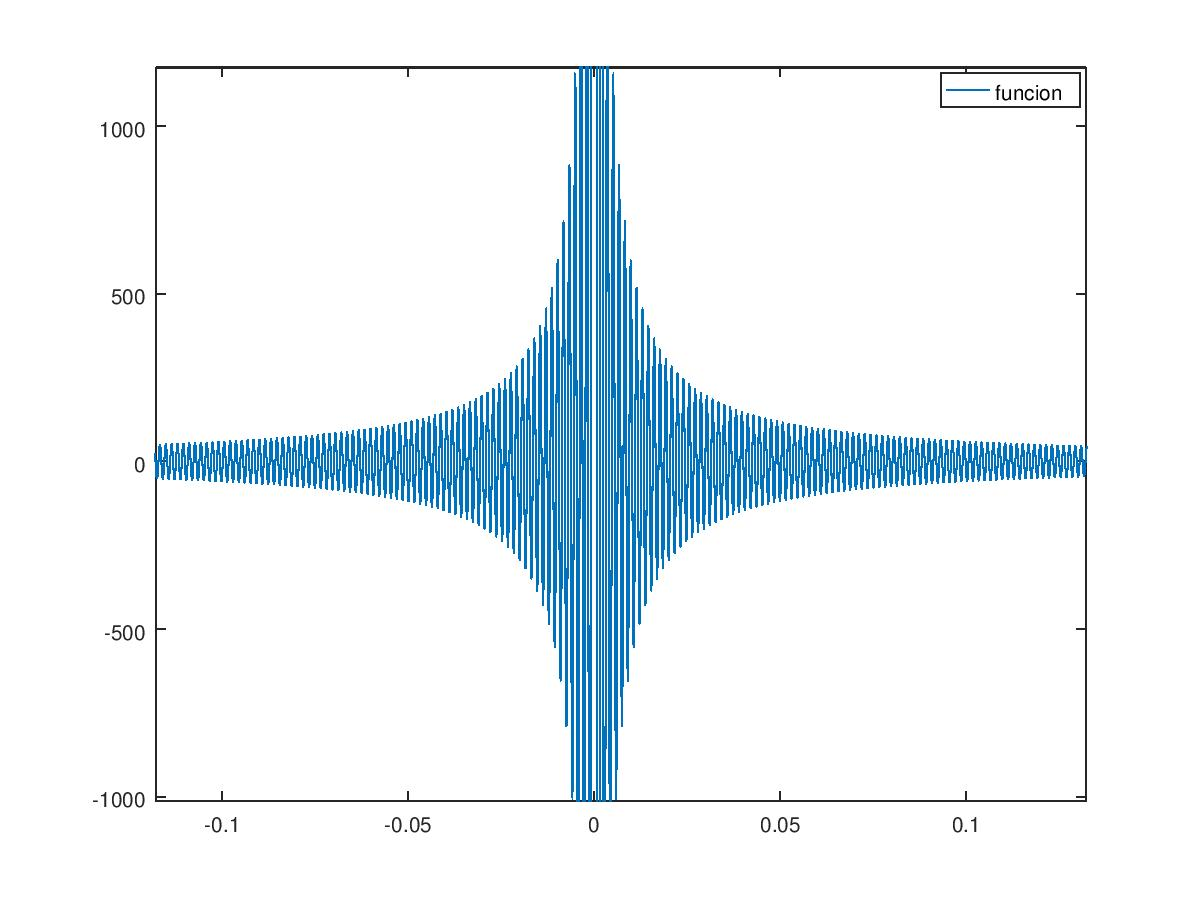
\includegraphics[width=1.2\textwidth]{figuras/funcion.jpg}}
	\caption{\(f(x)\)}
	\label{fig:funcion}
\end{figure}

\begin{figure}[H]
	\makebox[\textwidth][c]{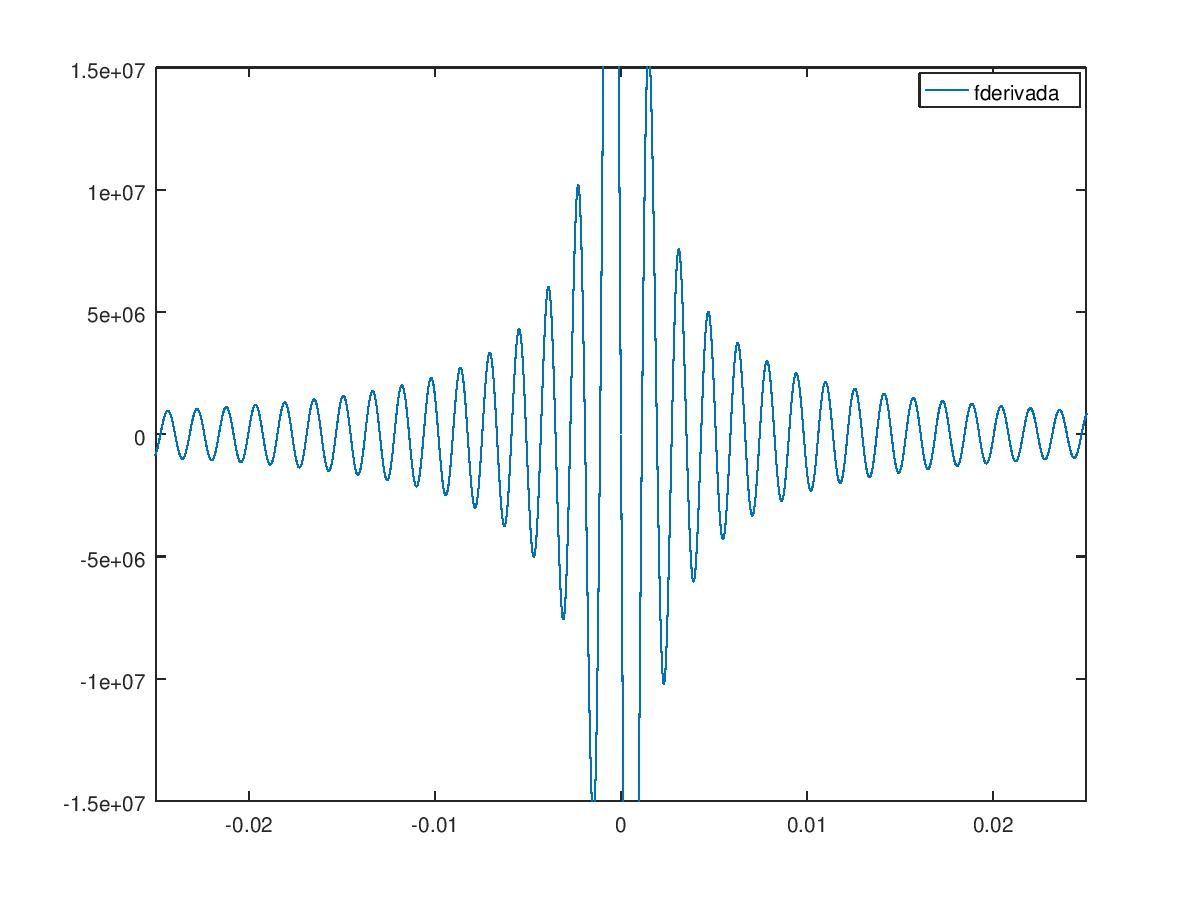
\includegraphics[width=1.2\textwidth]{figuras/funcionderivada.jpg}}
	\caption{\(f'(x)\)}
	\label{fig:funcionderivada}
\end{figure}

\begin{figure}[H]
	\makebox[\textwidth][c]{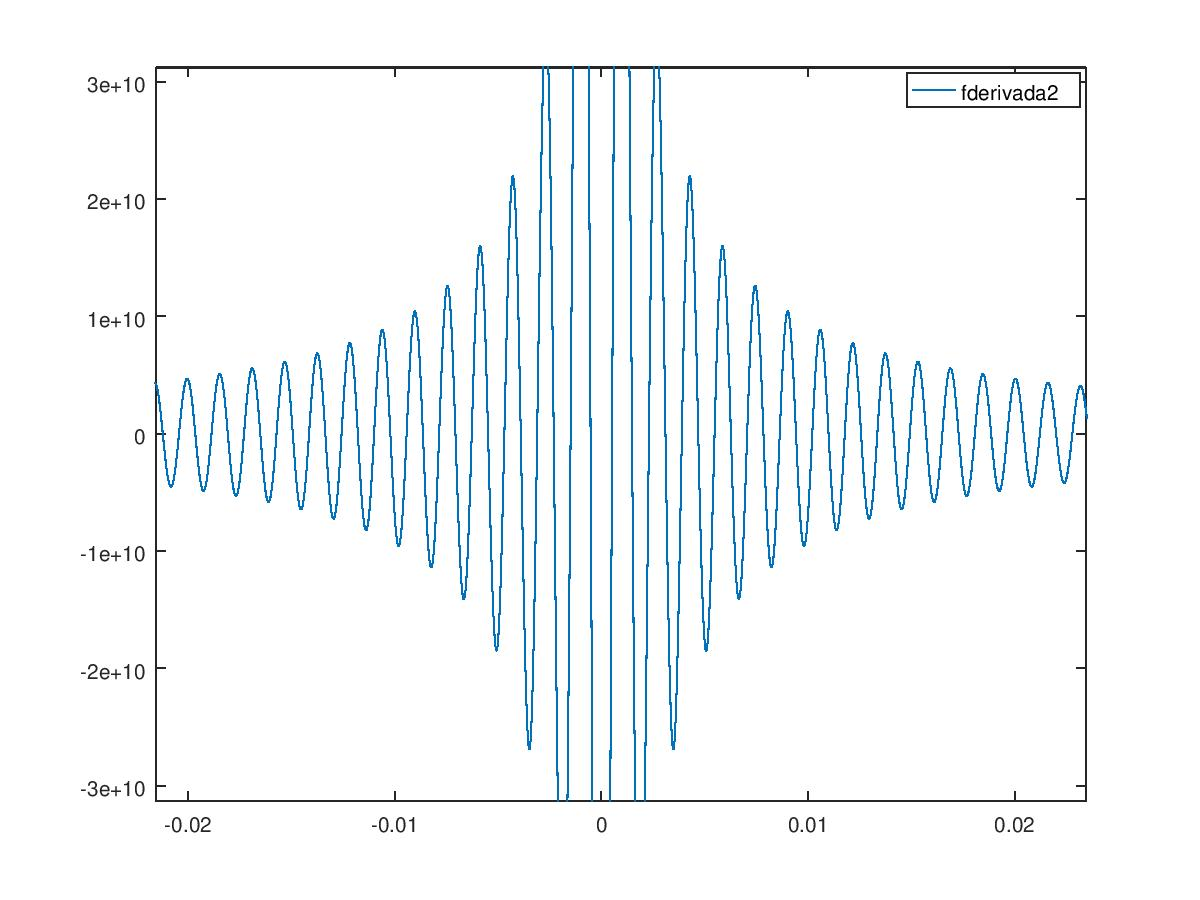
\includegraphics[width=1.2\textwidth]{figuras/funcionderivada2.jpg}}
	\caption{\(f''(x)\)}
	\label{fig:funcionderivada2}
\end{figure}

\subsection{Método de trapecios compuestos}

\subsubsection{Truncamiento de n}

\begin{figure}[H]
	\makebox[\textwidth][c]{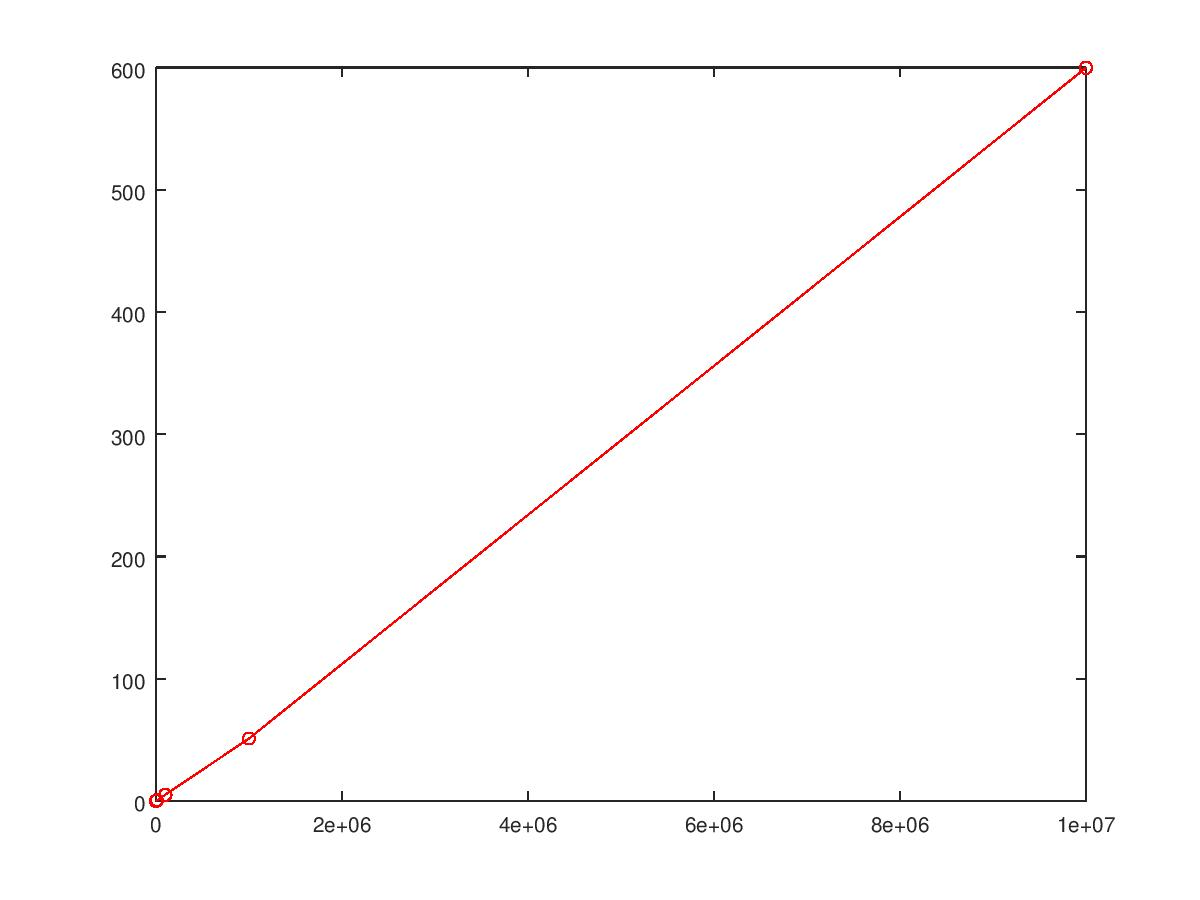
\includegraphics[width=1.2\textwidth]{figuras/calcularn.jpg}}
	\caption{Calculo de la integral para distintos n en funcion del tiempo}
	\label{fig:calcularn}
\end{figure}

\subsubsection{Precisión simple}

Haciendo los calculos se vió que n es igual a \texttt{241403216}, y luego se decidió truncar el número n a \texttt{5000000}. Para el n original la integral dió como resultado \texttt{\num{6.9458e+04}}, mientras que para n truncado dió \texttt{\num{6.9351e+04}}.

\subsubsection{Precisión doble}

Haciendo los calculos se vió que n es igual a \texttt{\num{2.4160e8}}, y luego se decidió truncar el número n a \texttt{5000000} para que sea un cálculo tratable. Para el n truncado la integral dió \texttt{\num{6.9458e+04}}.

\subsection{Condición del problema y término de estabilidad}
Con el método de perturbaciones experimentales llegamos a un cp respecto de alpha igual a \texttt{28.571} y respecto de beta igual a \texttt{4.9627}. El término de estabilidad es igual a \texttt{0.011211}

\begin{figure}[H]
	\makebox[\textwidth][c]{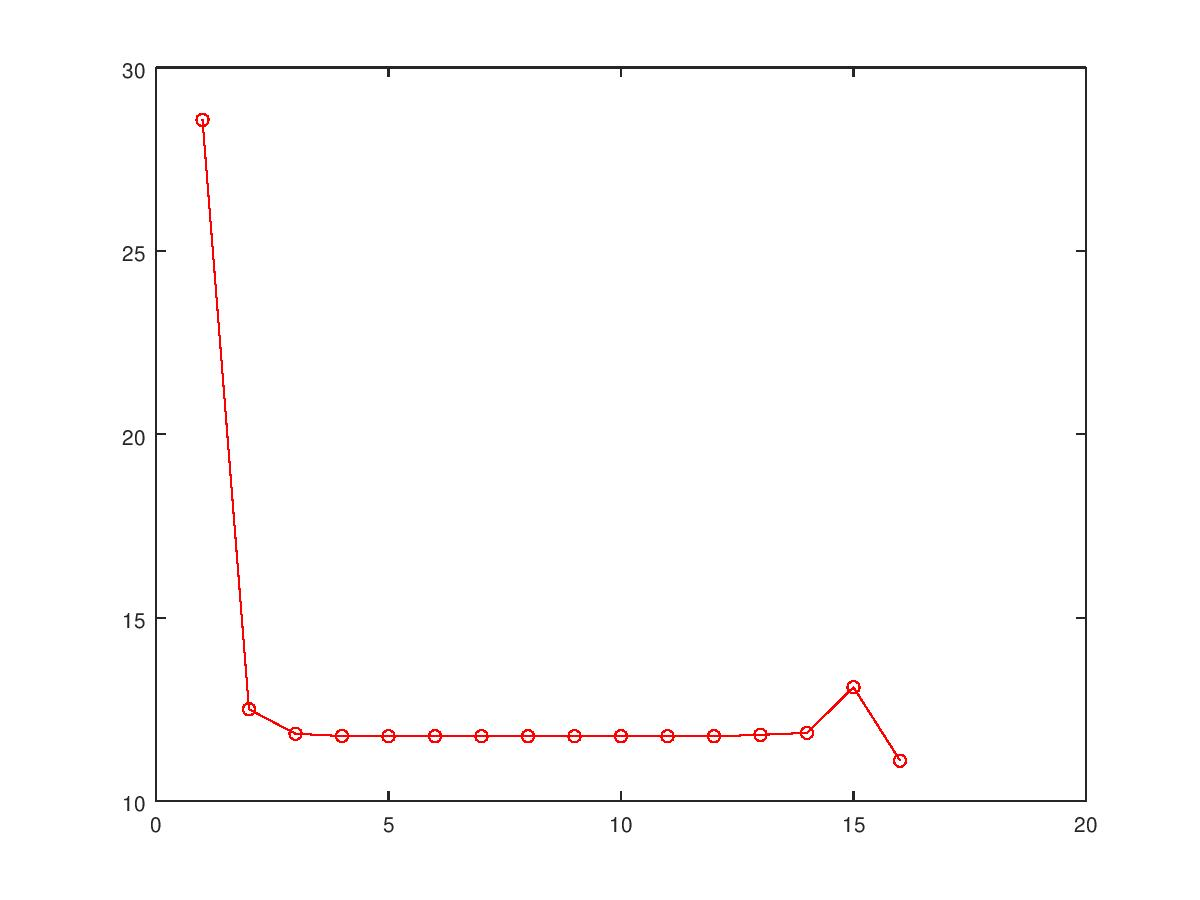
\includegraphics[width=1.2\textwidth]{figuras/cpsa.jpg}}
	\caption{Cp respecto de alpha por iteración}
	\label{fig:cpsa}
\end{figure}

\begin{figure}[H]
	\makebox[\textwidth][c]{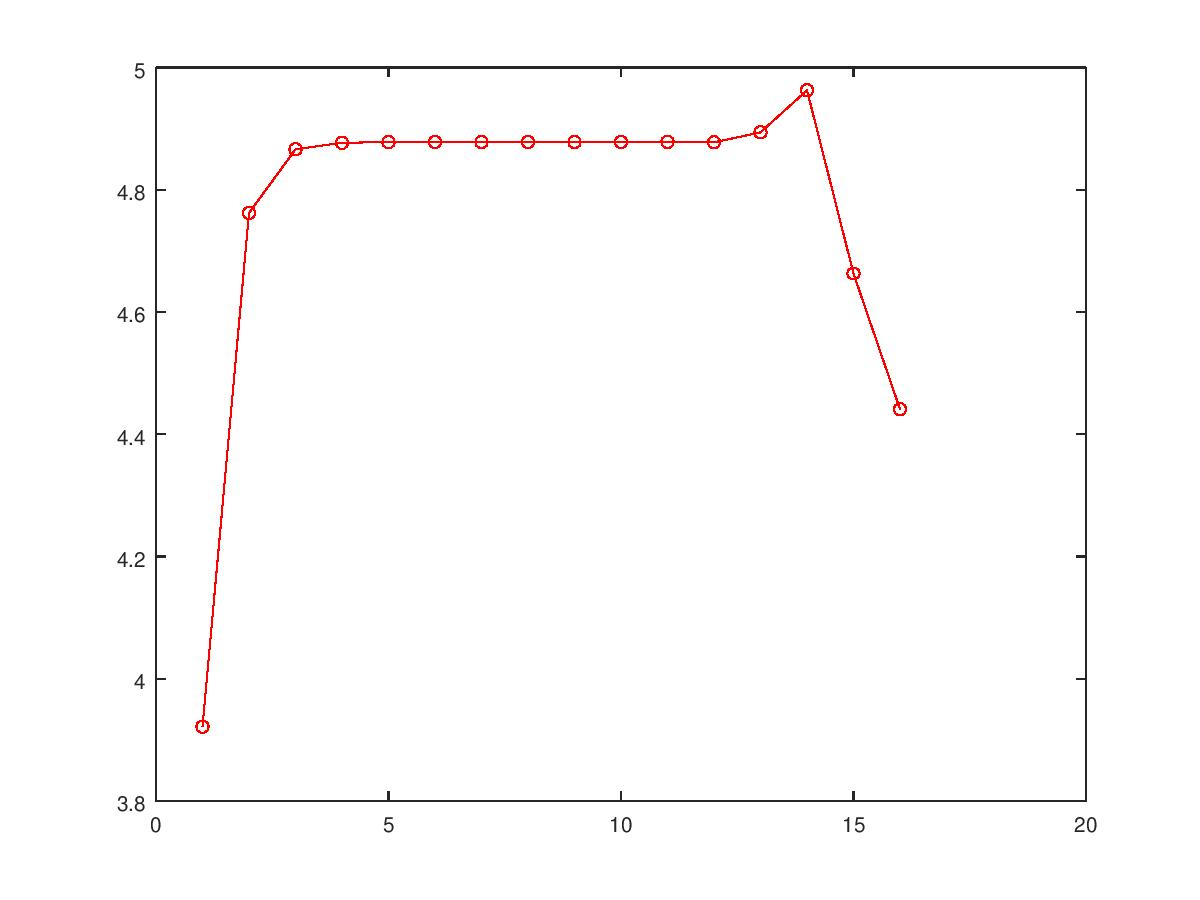
\includegraphics[width=1.2\textwidth]{figuras/cpsb.jpg}}
	\caption{Cp respecto de beta por iteración}
	\label{fig:cpsb}
\end{figure}

\subsection{Error total}

\subsubsection{Error inherente nulo}

\[ Et = Cp * r + Te * \mu_s + Etr \]

\[ Et < 0 + 1.1201*10^6 * 1*10^{-8} + 10^{-5} \]

\[ Et < 0.011211\]

\[ Et = Cp * r + Te * \mu_d + Etr \]

\[ Et < 0 + 1.1201*10^6 * 1*10^{-16} + 10^{-5} \]

\[ Et < 10^{-5}\]

\subsubsection{Error inherente acotado}

\[ Et = Cp * r + Te * \mu_s + Etr \]

\[ Et < 0.5*10^{-4} + 1.1201*10^6 * 1*10^{-8} + 10^{-5} \]

\[ Et < 0.011261\]

\[ Et = Cp * r + Te * \mu_d + Etr \]

\[ Et < 0.5*10^{-4} + 1.1201*10^6 * 1*10^{-16} + 10^{-5} \]

\[ Et < 6*10^{-5}\]

\section{Conclusiones}

Por empezar podemos concluir que el problema presentado esta mas cerca de estar bien condicionado (pues la condicion del problema no es tan lejana a 1) de lo que está de ser estable. Esto se debe al enorme valor que toma el termino de estabilidad debido a la gran cantidad de sumas que se realizan. Dichas sumas llevan atadas varios errores de redondeo que terminan produciendo el error mas importante del algoritmo. Si bien las cotas de error fueron calculadas con un error de maquina single dicho error puede ser acotado con una mejor precision de maquina (double) y llegar a un resultado de menor error. Concluimos que al aumentar la precision el error de redondeo disminuye y por lo tanto la cota de error total tambien lo hace. Distinto es disminuir la cantidad de cuentas a realizar (o dicho de otra forma, disminuir el valor de n) lo cual si bien disminuye el error de redondeo provocaría una mayor cota en el error de truncamiento. Por lo tanto a la hora de realizar calculos numéricos hay que trabajar con la mejor precisión posible siempre que queramos conseguir cotas de error lo mas pequeñas posibles.

Ahora bien, para un nivel de precisión doble el error de redondeo (al menos para el termino de estabilidad calculado) es basicamente despreciable contra el error de truncamiento. Esto sucede ya que al aumentar la precision, como bien dicho antes, se consiguen mejores cotas de error pues se pierde menos información en cada operación. Esto entonces nos lleva a pensar en que sería lógico buscar conseguir un error de truncamiento aun mas pequeño para que el error de redondeo deje de ser despreciable pero el resultado sea aún mas exacto. Pero esto tiene tambien sus, presentadas anteriormente, desventajas en tanto a tiempo de calculo no manejable. Se podría aumentar el numero de trapecios pero a costa de un tiempo de ejecucion mucho mas elevado y menos manejable. Ahora bien, considerando la cota de error inherente relativo, este error pasa a ser aquel de mayor relevancia pues su magnitud es mayor a la del mismo truncamiento. En este caso no tendría sentido intentar disminuir el error de truncamiento mucho mas pues, si bien no es totalmente despreciable, reducirlo no es rentable considerando la cantidad de tiempo necesario para realizar dichos calculos y tampoco es rentable pues no es siquiera el error mas relevante de todo el calculo.

Tambien podemos observar que, si bien el termino de estabilidad es muy grande, la diferencia en las medidas de la integral con precision simple y doble no estuvieron tan alejadas como esperado. Esperabamos que la diferencia fuera mayor pues los redondeos iban a afectar de forma mas directa al resultado teniendo menos precision a la hora de calcular pero evidentemente no fué así en nuestro caso. Pasamos gran parte del tiempo intentando identificar un error en el calculo de la integral en precision single sin poder lograrlo por lo que concluimos que o bien nuestra hipotesis era falsa o bien hay un error algoritmico en el calculo con dicho nivel de precision (el cual lamentablemente Octave no facilita su trabajo). Una pequeña conclusión a la cual llegamos luego de dicho tiempo fue que, logicamente, el termino de estabilidad depende directamente del algoritmo utilizado pues, a la hora de implementar el metodo de los trapecios, siempre realizamos sumas de numeros de magnitudes similares (pues, algoritmicamente hablando, calculamos el area de cada trapecio y los sumamos, en lugar de sumar todas las alturas de dichos trapecios y luego multiplicarlos por sus diminutas bases) y si bien los resultados no fueron tampoco demasiado diferentes, se pudo observar que usando un algoritmo distinto al que propusimos nosotros llevaba a un termino de estabilidad aún mas elevado y por lo tanto un error más elevado.

\newpage
\appendix
\section{Anexo I: Código Fuente}

El programa utilizado es GNU Octave, versión 4.2.2 y se procuró utilizar sintaxis compatible con Matlab, teniendo como única excepción la función \texttt{fplot} que brinda Octave para graficar funciones, despues de consultar con los docentes.

\lstinputlisting[language=Octave,title=\texttt{mu.m}]{src/mu.m}

\newpage
\lstinputlisting[language=Octave,title=\texttt{main.m}]{src/main.m}

\newpage
\lstinputlisting[language=Octave,title=\texttt{mainsingle.m}]{src/mainsingle.m}

\newpage
\begin{lstlisting}[language=Octave,title=Generación de graficos]
fplot(@f, [-0.02 0.02])
fplot(@fderivada, [-0.02 0.02])
fplot(@fderivada2, [-0.02 0.02])
\end{lstlisting}

\begin{lstlisting}[language=Octave,title=Truncamiento y gráfico de n]
function y = graficar_n()
    x = [1,10,100,1000,10000,100000,1000000,10000000];
    y = [];
    for n = x
        n
        tic;
        integral = calcular_area(n)
        y = [y,toc]; 
        printf("Tiempo = %ds\n\n",y(length(y)))   
    end
    plot(x,y,'o-r')
end
\end{lstlisting}

\newpage
\section{Anexo II: Resultados Numéricos}

\begin{lstlisting}[language=Octave,title=Corrida de \texttt{mu.m}]
>> mu
mu_simple =    1.0000e-08
mu_doble =    1.0000e-16
\end{lstlisting}

\begin{lstlisting}[language=Octave,title=title=Corrida de \texttt{main.m} con n original]
>> main
n =    2.4160e+08
Elapsed time is 12404.8 seconds.
ans =    6.9458e+04
\end{lstlisting}

\begin{lstlisting}[language=Octave,title=title=Corrida de \texttt{main.m}]
\begin{lstlisting}[language=Octave,title=Corrida de \texttt{mu.m}]
n_sin_truncar =    2.4160e+08
n =  5000000
integral =    6.9458e+04  
cpa =  28.571
cpb =  4.9627
te =    1.1201e+06
\end{lstlisting}

\begin{lstlisting}[language=Octave,title=title=Corrida de \texttt{mainsingle.m}]
>> mainsingle
n_sin_truncar =  241403216
n =  5000000
integral =    6.9351e+04
\end{lstlisting}

\begin{lstlisting}[language=Octave,title=Cálculos hechos para el criterio de truncamiento de n]
>> graficar_n
n =  1
integral =    6.9497e+04
Tiempo = 0.000295877s

n =  10
integral =    6.9459e+04
Tiempo = 0.000695944s

n =  100
integral =    6.9465e+04
Tiempo = 0.00530505s

n =  1000
integral =    6.9465e+04
Tiempo = 0.0516629s

n =  10000
integral =    6.9458e+04
Tiempo = 0.509583s

n =  100000
integral =    6.9458e+04
Tiempo = 5.11305s

n =  1000000
integral =    6.9458e+04
Tiempo = 51.1415s

n =  10000000
integral =    6.9458e+04
Tiempo = 599.773s
\end{lstlisting}


\begin{lstlisting}[language=Octave,title=Cps calculados para las distintas iteraciones]
cps_a =

Columns 1 through 11:

    28.571   12.500   11.834   11.772   11.765   11.765   11.765   11.765   11.765   11.765   11.765

Columns 12 through 16:

    11.765   11.768   11.857   12.212   11.102

cps_b =

Columns 1 through 11:

    3.9212   4.7614   4.8657   4.8763   4.8774   4.8775   4.8775   4.8775   4.8775   4.8775   4.8776

Columns 12 through 16:

4.8770   4.8683   4.7962   4.7740   4.4409
\end{lstlisting}


\newpage

\phantomsection 
\addcontentsline{toc}{section}{Bibliografía}
\renewcommand\refname{Bibliografía}
\begin{thebibliography}{9}

\bibitem{Gonzales} 
Gonzales, Hernan: 
\textit{Análisis Numérico, Primer Curso}
Buenos Aires: Nueva Librería, 2002.

\end{thebibliography}
\end{document}